\chapter{Versuch 1}
\label{chap:VERSUCH_1}


\section{Fragestellung, Messprinzip, Aufbau, Messmittel}
\label{chap:VERSUCH_1_FRAGESTELLUNG}

\subsection*{Fragesetellung}

Ziel war es eine Aufnahme von einen Grauwertkeil zu erstellen, damit dieser auf seine Bildfehler untersucht und später korrigiert werden kann.
Für einen besseren Vergleich soll zudem der Mittelwert und die Standardabweichung zu jeden der fünf Grauwerte ermittelt werden, damit diese mit den entsprechenden Werten des korrigierten Bilds verglichen werden können.

\subsection*{Messprinzip}
Der Grauwertkeiler stellt einen stufenweise Grauwertverlauf dar, 

\subsection*{Aufbau}

\subsection{Messmittel}
\begin{itemize}
\item Webcame (Asus USB2.0 UVC HD Webcam)
\item Grauwertkeil
\item Metermaß
\end{itemize}

\section{Messwerte}
\label{chap:VERSUCH_1_MESSWERTE}

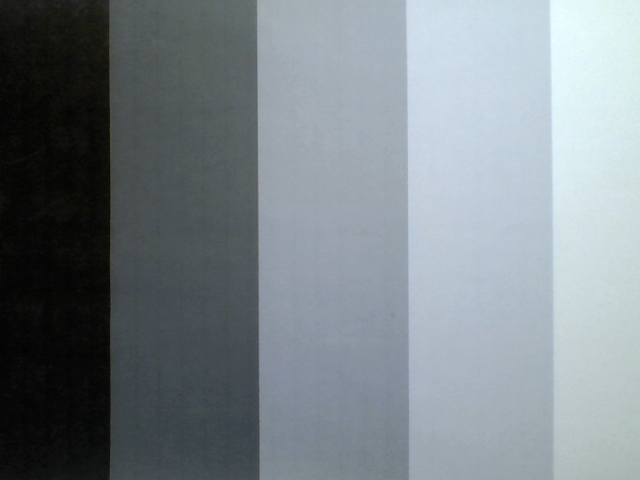
\includegraphics[scale=0.5]{media/grauwertkeil.png}
\captionof{figure}{Fig: Grauwertkeil, unbearbeitet}
\label{Fig:Grawertkeil}


\section{Auswertung}
\label{chap:VERSUCH_1_AUSWERTUNG}


\section{Interpretation}
\label{chap:VERSUCH_1_INTERPRETATION}